\documentclass[a4paper,10pt]{article}
%\documentclass[a4paper,10pt]{scrartcl}
\usepackage{hyperref}
% \usepackage{caption}
\hypersetup{pdfborder={0 0 0}}
\usepackage[all]{hypcap}
\usepackage{default}
\usepackage{graphicx}



\title{Pyceptron exercises}
\author{Olivia Guest}
\date{\today}

\begin{document}
\maketitle
\section{Running a perceptron on paper}
Yes, this can be done. 

\begin{figure}[hb]
 \centering
 \includegraphics{../slides/fig/perceptron_empty.pdf}
 \caption{A perceptron that you can run on paper.}
 \label{fig:perceptron}
\end{figure}
\section{Playing around with the network}
Firstly, let's have a go playing around, but hopefully not breaking, the network (see \autoref{fig:perceptron}). However, don't worry if you do break it, there is an infinite supply.

So let's have a go at looking at the code that makes it learn. Go to the part that says \texttt{def Train(self):}. This function, as I probably already explained, does a bunch of things that essentially implement the two basic equations. The first equation is that for calculating the activation of the output unit(s): 
\begin{equation}
y_j = f \left( \sum_1^N w_i \times x_i \right)
\end{equation} 
where $y_j$ is the (output) unit whose state we want to calculate, $N$ is the number of units on the previous layer, $w_{i}$ is the weight on the connection between $i$ and $j$, and $f$ is a function that the unit applies. In the code we can write that in many ways, just like you can say the same or similar things in natural language in a number of different ways. I decided on this:      \begin{verbatim}
              for i in range(N+1): 
                      y += x[i] * w[i]
                      
              y = f(y)
\end{verbatim} and hopefully you can guess what each variable is based on the equation. Please ask for help if something is not making sense straight away.

The second, and equally important equation, we need is the one that trains the weights:
\begin{equation}
\Delta w_i = \eta  ( d_j - y_j ) \times x_{i}
\end{equation} 
where $d$ is what we want $y$ to be given $x$, and $\eta$ is the learning rate. In other words $d$ is the target, $y$ is as before the output unit (or units), and $x$ are the unit units. As before, there are a number of different ways to say this in Python. Hopefully, my choice is a clear translation:
\begin{verbatim}
                   error = d[p][0] - y
                   
                   for i in range(N+1): 
                      w[i] += h * error * x[i]\end{verbatim} 

\begin{figure}[hb]
 \centering
 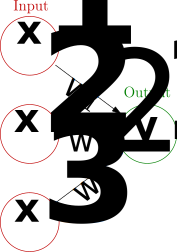
\includegraphics{../slides/fig/perceptron_maths.pdf}
 \caption{A perceptron}
 \label{fig:perceptron}
\end{figure}

Now that you have a slightly clearer idea (if not --- ask me or a demonstrator for clarification) of how the network works, have a go changing things to see what happens:

\begin{enumerate}
 \item Change the value of the learning rate $\eta$, aka \texttt{h}. What happens?
 \item Does printing out the values of the variables, e.g., \texttt{w}, \texttt{h}, \texttt{x}, \texttt{y}, etc. help you understand what's going on?
 \item What does \texttt{self.Draw()} do? Try commenting it out.
 \item What does the function \texttt{def Run(self):} (below \texttt{Train}) do?
 \item Can you spot similarities (and differences) between \texttt{Run} and \texttt{Train}? Imagine if it was called something less informative than  \texttt{Run}, would you still be able to reverse-engineer it?
\end{enumerate}




\section{Teaching the network logic}
To explore some of the  very basic uses of neural networks, we will first attempt to teach our perceptron logical operators. Logical operators were touched on in the first part of the workshop, when we talked about \textbf{not}, \textbf{and}, \textbf{or}, etc., and applied them to truth values (e.g., true and false).

Even though logical operators might seem very abstract, saying things like ``true \textbf{and} true is true'' is just a formalised way of saying much more common expressions such as ``I agree \textbf{and} you agree, therefore we both agree''. Natural language is full of such logical operations, for example when we ask questions, e.g., ``do you want sugar \textbf{or} milk in your tea?'' is equivalent to ``sugar \textbf{or} milk'' in formal logic. Such formalisation is useful because it is an easy way to avoid ambiguity which is required when programming.

\subsection{Not}

The first logical operator we will teach our perceptron is the \textbf{not} operation. This requires one input unit and one output unit because negation (a synonym for not) is applied to one variable (or in our case input unit) at a time. So when we give the network a 0 we want it to return a 1, and when we give the network a 1 we need a 0 on the output. That means our training patterns are 0 and 1, and our targets are 1 and 0, in that order. \autoref{tbl:not} represents our patterns and their required targets. 
%modify this section to say where in the code you need to edit stuff

\begin{table}[hb]
 \centering
 \begin{tabular}[t]{cc}
Input & Output\\ \hline
0 & 1\\
1 & 0
\end{tabular} \caption{Truth table for logical \textbf{not}.}
 \label{tbl:not}
\end{table}

Once you have made the required changes, run the network to see what happens and how long it takes to train. 

\ \\ Can the network learn \textbf{not}?    Yes / No                                               
                                                     

\subsection{And}

Now let's teach it something a little more complex, the most basic form of logical \textbf{and} is that with two inputs (e.g., false \textbf{and} true is false) and it always has one output. Meaning that the network needs to learn the input-output mapping given in \autoref{tbl:and}. By looking at \autoref{tbl:and}, you might notice that now there are three units, two input units and the same number of output units as before. So we need to modify the network to have two input units, leaving the single output unit untouched. Thankfully, the code can figure out the number of input and output units required based on the patterns and targets you give it. This is something I wrote myself, if you want to see how that is done see, but do not get bogged down with understanding this  %modify this section to say where in the code you need to edit stuff
Once the patterns and targets are set, run the network like before and see what happens.

\ \\ Can the network learn \textbf{and}?    Yes / No                                             

\begin{table}[ht]
 \centering
 \begin{tabular}[t]{ccc}
Input 1 & Input 2 & Output\\ \hline
0 & 0 & 0\\
0 & 1 & 0 \\
1 & 0 & 0 \\
1 & 1 & 1 \\

\end{tabular} \caption{Truth table for logical \textbf{and}.}
 \label{tbl:and}
\end{table}

\subsection{Or}

Now let's do the same for \textbf{or}. Logical \textbf{or} returns a 1, or true, if either input is on. In other words, it only returns 0 when neither are 1, as shown in \autoref{tbl:or}. Remember that at any point you can check what any logical operator does directly in the Python shell, e.g., by typing \texttt{False or True}, Python will say \texttt{True} (corresponding to the 3rd line of \autoref{tbl:or}).

\ \\ Can the network learn \textbf{or}?    Yes / No                                             

\begin{table}[ht]
 \centering
 \begin{tabular}[t]{ccc}
Input 1 & Input 2 & Output\\ \hline
0 & 0 & 0\\
0 & 1 & 1 \\
1 & 0 & 1 \\
1 & 1 & 1 \\

\end{tabular} \caption{Truth table for logical \textbf{or}.}
 \label{tbl:or}
\end{table}

\subsection{Xor}
Things start to become interesting when we teach the network \textbf{xor}, also known as exclusive or. Like its namesake \textbf{or}, \textbf{xor} returns true when either one or the other inputs are true, \emph{but it does not} return true when both are true (compare \autoref{tbl:xor} with \autoref{tbl:or}).  


In Python one way of specifying \textbf{xor} is by using \texttt{(a and not b) or (b and not a)}. You do not need to know this to program the network, because the network figures out how to map inputs onto outputs itself, or at least tries to...

\begin{table}[ht]
 \centering
 \begin{tabular}[t]{ccc}
Input 1 & Input 2 & Output\\ \hline
0 & 0 & 0\\
0 & 1 & 1 \\
1 & 0 & 1 \\
1 & 1 & 0 \\

\end{tabular} \caption{Truth table for logical \textbf{xor}.}
 \label{tbl:xor}
\end{table}


\ \\ Can the network learn \textbf{xor}?    Yes / No   
\ \\
\end{document}
